This chapter presents methods used to evaluate the system and the results collected evaluating the system. 

\section{Methods}
\subsection{User Survey}

The system is measured by doing user surveys on the end users. In our user survey we have coaches’ rating how much they agree with a statement on a Likert-scale. The statements compare the system against other systems in use at Alfheim today. The Likert-scale chosen is a 5 point scale from \textit{strongly disagree} to \textit{strongly agree}.\footnote{http://www.simplypsychology.org/likert-scale.html}. In short it will let each individual to note how much they disagree or agree with a particular statement.

Including to this external people not in the Tromsø IL system. This includes Ruben Yttergård Jenssen playing in the national soccer team for Norway and FC Kaiserslatern in 2. Bundesliga, and Lars Tjærnås, a previous coach and now football expert in Canal+ also writing for 100‰ fotball.

\section{Experiments and Results}

\subsection{Test data and Assessors}

In the tests Tromsø IL academy coaches has been evaluating the system. In the evaluation phase the database had been populated with data from Tromsø IL and Strømsgodset Toppfotball matches. Only attacks from these two teams have been used in the evaluating process. A total of 34 attacks have been captured for Strømsgodset over 5 matches. For Tromsø a total of 42 attacks have been captured over 9 matches. Figure \ref{fig:matches_regged} lists all matches. Some matches include data from other teams than Tromsø and Strømsgodset. They have not been taken into consideration in the evaluating process.

\begin{figure}[ht!]
\centering
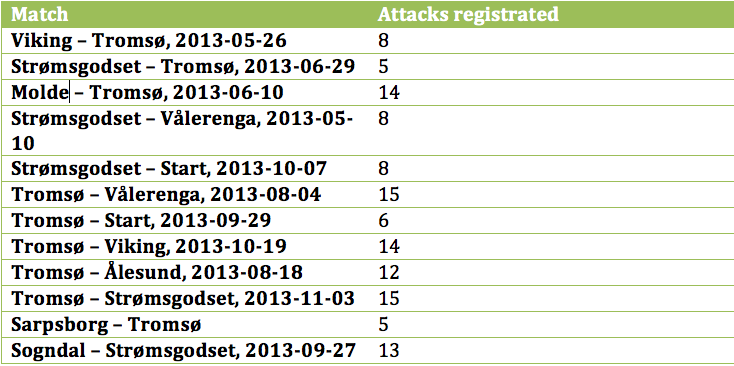
\includegraphics[width=1\textwidth]{images/general/matched_regged.png}
\caption{Matches that have been captured and persisted into the database}
\label{fig:matches_regged}
\end{figure}

\subsection{SAT as a tool for opponent analytic}
% SAT gives you valuable information about opponents that the current systems you use today don’t provide

In this User Servey the assessors where asked how SAT is as a complementary opponent analytic tool. In the requirement process we specified that the system should to be a complementing tool and not a direct replacement of the systems in use. The results shows that most of the assessors values what the system provides. 

Assessors not in the Tromsø IL system do not necessarily use or have experience with an existing tool. Therefor the statement was re-phrased. The assessors were asked how SAT is as an opponent analytic tool, a stand-alone product. The results shows

From these results we can conclude that the end-users view the Soccer Analytic Tool as a good system to complement with for opponent analytic. 

\subsection{SAT as a tool for identifying key players}

In this User Servey the assessors where asked how SAT is as a tool for identifying key players in a soccer team. This was one of the main goals of the system. We can see from the results of the User Servey that the system identifies key players exceptional well. All votes for ¨strongly agree¨. 

\subsection{UI-performance}

\section{Discussion}
\subsection{Input}

Perhaps the biggest limitation of the system is that it requires manual work to be functional. The system requires a lot of manually work to be operational as an opponent analytic tool. Up to one hour is the normal time spent capturing all data for a match with the current capture interface. On average, teams across the top four top leagues (La Liga, Premier League, Serie A and Bundesliga) took about 13 shots per match, measured in the 2010/11 season \cite{soccerbynumbers}. This means you will have possible have 26 attacks to capture (not all shots can be seen as an attempt on goal).

As mentioned in section \ref{sec:capprocess} you have to store the players by their ID. IDs are only found in the database. Instead of this a player selector interface could have been developed letting you just click on a image of the player involved. We suggest you can save up to 20 minutes by having this feature added.

There is minimal quality checking of the input data except from the match view page that lists every attack captured, meant for external operators to verify the data. Other than that you have to trust the operator that is capturing match data. The input is to some degree subjective for some data like identifying breakthroughs. In some situations one operator may say that it was a breakthrough and another wouldn't agree. This may not be the biggest problem if you set some rules to follow for the operators.

\subsection{Interfaces}

One comment of a end users was about the graphical components on the client. Improving the graphical components would increase the overall experience of the system. This has not been one of the main focuses during the development of the system.

\subsection{Scalability}

